次に,各ステップ間の平均移動距離$\phi$を計算し,それが$N$によってどのように変化するかを図\ref{fig:f24}に示した。このとき$X_{i}$のもつ点の数$S=20$,クラスタ化閾値$r=0.07$とした。
\begin{figure}[H]
    \begin{center}
        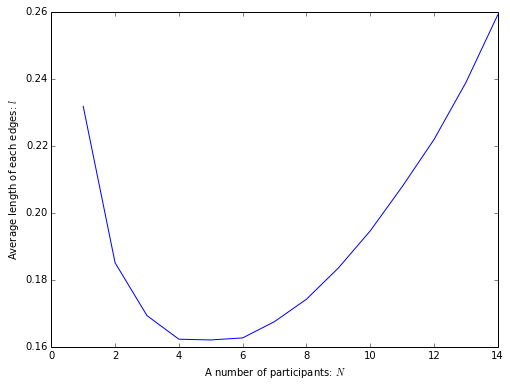
\includegraphics[width=10cm]{../img/N_l_2.png}
        \caption{ステップ間距離の平均値$\phi$と$N$の間の関係}
        \label{fig:f24}
    \end{center}
\end{figure}
このグラフを見て分かるように,$\phi$は$N$の関数として見たとき下に凸な関数となっている。
このようなグラフとなるのは,先程まで考えたように$N$が増えると点の密度が大きくなり,同じ$r$でもクラスターの融合が進むので,結果的にクラスター間の距離は離れることになるということ,それから点の密度が小さいときには,クラスターは形成されにくいが,かわりに各点間の距離は広がるために各ステップ間の距離も大きくなる,と説明できる。

ここまで考えてきた各ステップ間の距離というのは,はじめに設定としてイメージしていた会議を思い浮かべると,意見間の差異を表すことになる。
この値が小さいということは,選択された意見の間につながりが見られること,妥当な思考の過程によって次の意見が提出されたことを意味していると見ても良いかもしれない。
逆にこの値が大きい時には,意見と意見の間の関連が小さいということを意味しており,それゆえ選択された意見間は,およそつながりがなさそうな意見になっていると言うことができる。
つまり突拍子もない意見が提出されている,ということであり,生産的な会議になっているとは考えにくい。
